\documentclass[crop,tikz,convert={outext=.svg,command=\unexpanded{pdf2svg \infile\space\outfile}},multi=false]{standalone}[2012/04/13]
%\usetikzlibrary{...}% tikz package already loaded by 'tikz' option

%%% Tikz libraries and definitions
\usetikzlibrary{intersections}
\usetikzlibrary{arrows}
\usetikzlibrary{calc}                 % coordinate calculations ($ n1 + (0:1cm) $)

% Common style for Simulink blocks.
\tikzstyle{block} = [rectangle, rounded corners, minimum width=3cm, minimum height=0.8cm,text centered, thick, draw=black]
% Common style for connectors. 
\tikzstyle{arrow} = [->,>=stealth',font=\scriptsize,rounded corners]

% Some distances to share between figures.
\newcommand{\shift}{0.28cm}
\newcommand{\bigshift}{1cm}

\begin{document}


  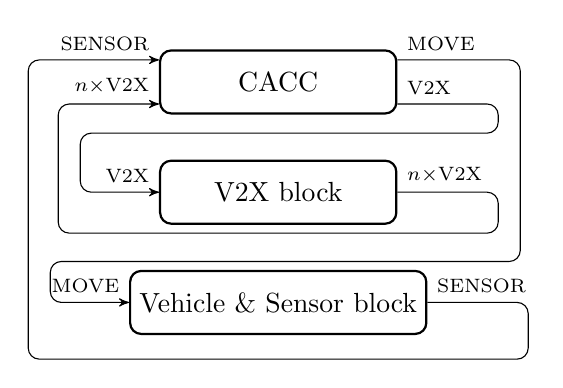
\begin{tikzpicture}[node distance=1.4cm]
  
  %\draw[help lines] (-2,-2) grid (2,2);

  \node (cacc) [block] {CACC};
  \node (v2x)  [block, below of=cacc] {V2X block};
  \node (vehicle) [block, below of=v2x] {Vehicle \& Sensor block};

  % CACC - V2X
  \draw [arrow] ([yshift=-\shift]cacc.east) node [anchor=south west] {V2X} -- % a little below east
                 ++(\bigshift + \shift,0) |-               % ++ is relative coordinate, |- means connect vertically-then-horizontally
                 ([xshift=-\bigshift,yshift=0.75cm]v2x.west) |-  % left knee
                 (v2x.west) node [anchor=south east] {V2X};

  % CACC - Vehicle
  \draw [arrow] ([yshift=\shift]cacc.east) node [anchor=south west] {MOVE} -- 
                ++(\bigshift + \shift + \shift, 0) |- 
                ([xshift= - \bigshift,yshift=0.8cm-\shift]vehicle.west) |- 
                (vehicle.west) node [anchor=south east] {MOVE};

  % V2X - CACC
  \draw [arrow] (v2x.east) node [anchor=south west] {$n \times$V2X} -- 
                ++(\shift + \bigshift,0) |-
                ([xshift=-\shift - \bigshift, yshift=-0.8cm+\shift]v2x.west) |- 
                ([yshift=-\shift]cacc.west) node [anchor=south east] {$n \times$V2X};

  % Vehicle - CACC
  \draw [arrow] (vehicle.east)  node [anchor=south west] {SENSOR} -- 
                ++(\shift + \bigshift,0) |-
                ([xshift= - \shift - \bigshift, yshift=-1cm+\shift]vehicle.west) |-
                ([yshift=\shift]cacc.west)  node [anchor=south east] {SENSOR};

  \end{tikzpicture}

\end{document}

